\chapter{Teorie}
\label{chap:teorie}

    V této části bych rád uvedl všechny základní součásti, na kterých má práce
    stojí, a~také bych se rád zmínil o způsobech, jak řeší ovládání robota
    jiní. Nejprve je nutné zjistit, jaké vlastnosti má robot e-puck, abychom
    pak dále mohli posoudit do jaké míry využíváme jeho předností a také
    zhodnotit využitelnost práce v~praxi.

    Popis e-puck robota je v sekci \ref{e-puck robot}. Také je nutné zmínit
    způsoby komunikace, jaká úskalí přináší oddělení kontrolního programu od
    hardware a jak se dají mírnit rizika z tohoto plynoucí, tím se zabývá sekce
    \ref{sync/async}. V sekci \ref{existujici prace} se podíváme na jiné
    projekty, které se zabývají ovládáním robota. Nakonec v části
    \ref{specifikace} je k nalezení specifikace vytvořené e-puck knihovny.

    \section{E-puck robot}
    \label{e-puck robot}
    E-puck je miniaturní robot stvořený pro výukové účely na akademické úrovni.
    Vytvořen byl v EPFL (Ecole Polytechnique Fédérale de Laussanne) v roce
    2004. Celý projekt je založen na principu otevřeného hardware a open
    source, což znamená, že všechny dokumenty a schémata jsou dostupná pod
    svobodnou licencí umožňující komukoli využívat e-puck robota na maximum a
    vyvíjet pro něj ať už software, anebo např. hardwarové nadstavby.

    \renewcommand\listingscaption{Obrázek}
    \begin{listing}
        \begin{center}
            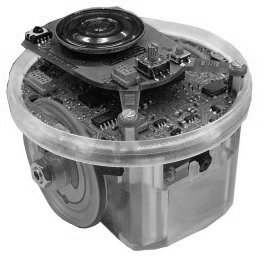
\includegraphics[scale=0.5]{e-puck.jpg}
            \caption{E-puck robot}
        \end{center}
    \end{listing}
    \renewcommand\listingscaption{Zdrojový kód}

    E-puck robot byl vytvořen s několika kritérii \cite{bonani}:
    \begin{itemize}
        \item Stolní velikost -- možnost experimentovat s robotem přímo u
        počítače je velmi výhodná pro studenty. Pokud se za optimální velikost
        pracovní plochy považuje 10-ti násobek velikosti robota, tak e-puck se
        svým průměrem 75mm je ideální pro použití na stole.

        \item Široké spektrum použití -- robota je možné použít nejen pro výuku
        robotiky, ale také například pro výuku zpracování obrazu nebo zvuku,
        programování vestavěných systémů, automatizace atd. Toho je docíleno
        velkým spektrem senzorů.

        \item Uživatelská přívětivost -- při vytváření rozhraní by vždy měl být
        kladen důraz na jednoduchost. Rozhraní by mělo být intuitivní a
        důkladně zdokumentované, aby se zrychlil proces učení.

        \item Možnost dálkového ovládání -- robot v sobě obsahuje Bluetooth
        modul, který se pro něj chová jako sériové zařízení, přes které dokáže
        komunikovat s počítačem.
    \end{itemize}

    Součástí robota je velká škála senzorů a akčních členů. Srdcem robota je
    mikrokontrolér s obvodem dsPIC. Skládá se z 16bitového procesoru dsPIC
    30F6014A a jednotky pro zpracování signálu. Procesor má frekvenci 64 MHz, 8
    kB RAM a~144 kB flash paměti. Robot obsahuje následující senzory:

    \begin{itemize}
        \item Infračervené (IR) senzory -- po obvodu robota je 8 IR senzorů. Měří
        buď vzdálenost od překážek, anebo intenzitu okolního světla. Jedná se o
        základní senzory využívané pro pohyb mezi překážkami.

        \item Akcelerometr -- 3D akcelerometr slouží k získání vektoru
        zrychlení robota. Může být použit pro spoustu experimentů (měření
        náklonu, zrychlení, detekce nárazu, pádu, \ldots).

        \item 3 mikrofony -- mikrofony jsou 3, aby se daly použít k triangulaci
        zdroje zvuku. Velikost dat získaných z mikrofonů je ovšem na kapacity
        robota příliš a proto je nutné použít jednotku pro zpracování signálu
        (DSP). Bez jejího použití můžeme získat alespoň naměřenou hlasitost.

        \item Barevná kamera -- v přední části robota je kamera s rozlišením
        640x480, bohužel kvůli paměťovým omezením robota je možné získat pouze
        část obrazu. I tak je ale možné ji použít pro experimenty s počítačovým
        viděním.
    \end{itemize}

    Samotné senzory by samozřejmě byly bez užitku, kdyby robot neměl žádné
    akční členy. Studenti mohou využít následujících komponent:
    \begin{itemize}
        \item 2 krokové motory -- slouží pro pohyb robota, mají rozlišení 1000
        kroků za jedno otočení kola.

        \item Reproduktor -- ve spojení s mikrofony může sloužit pro
        dorozumívání s~jinými roboty, také jde o výhodný způsob interakce s
        uživatelem.

        \item 8 LED -- diody jsou rozmístěné po obvodu robota. Slouží jako
        vizuální rozhraní pro uživatele, anebo pro jiného robota.

        \item Zelená dioda uvnitř robota -- hlavním jejím posláním je zkrášlit
        robota, ale také může být použita pro interakci s jinými objekty.

        \item Přední dioda u kamery -- tato LED nevytváří rozptýlené světlo,
        ale paprsek, který je možné použít dohromady s kamerou pro odhadování
        vzdálenosti k~překážkám, když IR senzory nestačí.
    \end{itemize}

    Ovládání e-puck robota je možné řešit několika způsoby. V první řadě
    existuje kompatibilní GCC kompilátor, takže je možné psát řídící program,
    který bude vykonáván přímo uvnitř robota, v programovacím jazyku C. Výrobce
    navíc dodává knihovnu s intuitivním rozhraním pro ovládání všech součástí.
    Tento přístup má ovšem několik nevýhod. Cyklus vývoje programu je pomalý,
    kvůli každé změně v~programu je třeba spustit kompilaci na počítači, dále
    nahrát program do robota a~teprve pak je možné změnu vyzkoušet. Dalším
    problémem je výkon robota, který nemusí stačit pro složitější výpočty.

    Lepším způsobem se tedy zdá využívat program v robotovi pouze pro
    vykonávání příkazů, které jsou naplánovány v počítači. To je přístup,
    kterým se zabývá tato práce. Získáme tím jednu obrovskou výhodu, kterou je
    výpočetní síla stolního počítače, na druhou stranu s ní ovšem musíme
    přijmout i břímě problémů s~komunikací.

    \section{Synchronní / asynchronní komunikace}
    \label{sync/async}

    Pojem komunikace ve světě počítačů označuje předávání dat mezi dvěma
    programy nebo zařízeními. Příkladem může být komunikace mezi webovým
    prohlížečem a http serverem při stahování stránky, počítačem a tiskárnou
    při tisku, atd. Průběh komunikace je vždy velmi podobný, jedna strana pošle
    zprávu obsahující požadavek, druhá strana zprávu přijme a zpracuje. Pokud
    ke zpracování potřebuje další informace, pošle odesílateli jako odpověď
    žádost o jejich dodání a tak si zúčastněné strany vymění role a situace se
    opakuje.

    Přenos zprávy ovšem může zabrat netriviálně mnoho času a tak je tu problém,
    co bude dělat odesílatel zprávy, zatímco čeká na odpověď. Tady dochází k
    rozdělení na synchronní (nebo také blokující) a asynchronní (neblokující)
    komunikaci. Popisem synchronní komunikace se zabývá sekce \ref{sync},
    popisem asynchronní komunikace sekce \ref{async}. A nakonec je v sekci
    \ref{comm-epuck} popsáno jak byly tyto principy uplatněny v praxi.

    \subsection{Synchronní komunikace}
    \label{sync}

    Při synchronní komunikaci program po odeslání zprávy pozastaví vykonávání
    dalších instrukcí a čeká dokud nedostane odpověď. Tento přístup je velmi
    jednoduchý na implementaci (většinou se jedná o zavolání metody, která bude
    čekat, dokud neobdrží zprávu), není problém s inkonzistencí dat (než bude
    program pokračovat v činnosti, obdrží všechny informace).

    Překážkou pro synchronní komunikaci jsou ovšem ztráty zpráv při přenosu.
    Může dojít k chybě při přenosu dat a ke ztrátě odeslané zprávy, anebo
    příchozí odpovědi. Stejně tak se může stát, že adresát zprávy na ni nijak
    neodpověděl. V~takovýchto případech lehce dojde k tzv. dead-locku, kdy bude
    odesílatel čekat na zprávu, která nikdy nepřijde, a tak nebude moci
    pokračovat v dalších výpočtech.

    Dochází také k mrhání procesorovým časem. Čas strávený čekáním na odpověď
    by mohl být smysluplně využit. Typickým příkladem je grafické rozhraní, kde
    je potřeba zaručit interakci a nereagování na akce uživatele je ukazatelem
    špatně napsané aplikace. Ale nemusí jít jen o složité aplikace s grafickým
    rozhraním, čas strávený čekáním lze využít například pro zpracování
    již přijatých dat a díky tomu zvýšit jejich průtok.

    \subsection{Asynchronní komunikace}
    \label{async}

    Pokud je po programu požadována interaktivita, anebo komunikace není jeho
    jediným úkolem a musí zvládat například obsluhovat více blokovaných
    spojení, tak synchronní komunikace přestává stačit.

    Asynchronní komunikace řeší některé problémy komunikace synchronní. Po
    odeslání zprávy program pokračuje ve vykonávání instrukcí, nečeká na
    odpověď. Může si ale kdykoli zkontrolovat, zda-li už nepřišla odpověď a~pak
    ji teprve načíst a zpracovat. Speciálním případem je komunikace řízená
    událostmi (event-driven), kdy je pro zpracování události přijetí zprávy
    určena funkce, která je automaticky spuštěna, bez přímé intervence
    programátora.

    Asynchronní komunikace velmi zjednodušuje vyřešení problémů se ztrátou
    zpráv. Protože program se musí sám podívat jestli nepřišla odpověď, tak si
    také může pamatovat, kdy byla odeslána zpráva a pokud odpověď nedorazí do
    určitého času, tak zprávu prohlásí za ztracenou a může se pokusit ji poslat
    znova.

    I asynchronní komunikace má své problémy. Odpovědi na zprávy nemusí přijít
    ve stejném pořadí, v jakém byly odeslány. Tento problém musí řešit
    například protokol TCP/IP. Řešením je zprávy posílat s pořadovým číslem a
    toto číslo přidat i k odpovědi. Pak je velmi snadné příchozí zprávy seřadit
    podle pořadí, v~jakém jsou požadovány.

    \subsection{Komunikace v e-puck knihovně}
    \label{comm-epuck}

    V této práci je uživateli knihovny dána možnost vybrat si mezi komunikací
    synchronní a asynchronní. Synchronní komunikace je určena pro rychlé
    prototypování a interaktivní ovládání robota. Uživatel může zadávat příkazy
    a~dívat se, jak na ně robot reaguje. Tady je výhodná transparentnost
    synchronního přístupu. Naopak pro psaní kontrolních programů je větší důraz
    kladen na spolehlivost. Knihovna zajistí, že příkaz opravdu dojde, v
    nejhorším případě upozorní uživatele na skutečnost, že robot je
    neovladatelný (může se to stát, třeba pokud mu dochází baterie).

    Výhodou je, že firmware v e-pucku robotovi je z důvodu hardwarových omezení
    napsán synchronně. Na začátku je vždy zavolána funkce pro čtení z~Bluetooth
    spojení, zablokuje vykonávání dalších instrukcí a čeká, dokud nedojde
    příkaz, který by se mohl zpracovat. Po provedení příkazu robot pošle
    odpověď a opět začne čekat na příkazy z počítače. Tedy vždy platí, že robot
    buď zpracuje zprávy v takovém pořadí v jakém byly poslány, anebo případně
    některé z nich vynechá.

    Při asynchronní komunikaci tedy stačí mít frontu příkazů a kontrolovat, že
    je robot postupně vykonává. To je také důvod proč jsou zprávy opatřeny
    kódem příkazu a pořadovým číslem. Kód příkazu je jeden znak, který určuje o
    jaký příkaz se jedná (např. změna rychlosti nebo nastavení LED). Pořadové
    číslo je v podstatě také jeden znak, jeho číselná hodnota v ASCII kódování
    určuje pořadové číslo zprávy. Z toho samozřejmě vyplývá, že pořadová čísla
    nejsou unikátní. Ovšem mezi dvěma zprávami, které potenciálně mohou mít
    stejný kód i stejné pořadové číslo, musí být posláno tolik jiných zpráv
    (pořadí je určeno znaky anglické abecedy, takže by jich muselo být 52), že
    pravděpodobnost záměny těchto dvou je velmi malá (musely by se ztratit
    všechny zprávy mezi nimi a v takovém případě už je komunikace opravdu velmi
    nestabilní).

    Díky přidaným informacím ke zprávě není problém poslat např. více zpráv,
    které mění rychlost robota, za sebou. Je zajištěno, že budou provedeny
    všechny příkazy postupně a robot skončí v očekávaném stavu. Ukázkovou
    situací může být robot, který stojí před překážkou, chceme aby se otočil a
    pokračoval v jízdě dopředu. Pokud by se ztratil první příkaz, tak robot
    pojede dále proti překážce, pokud by se ztratil druhý příkaz, tak se bude
    robot pouze točit na místě. Díky danému pořadí příkazů se nemusíme
    takovýchto situací bát.

    \section{Existující práce}
    \label{existujici prace}

        Existuje mnoho prací, které se zabývají ovládáním robota. V sekci
        \ref{webots} bude ukázán komerční simulátor Webots. K němu vznikla také
        kniha Cyberbotics' Robot Curriculum (sekce \ref{curriculum}). Další
        kniha, která se zabývá robotikou a programovacím jazykem Python je
        Learning Computing With Robots (sekce \ref{learning-computing}). U
        Webots nekončí seznam existujících simulátorů, Evorobot* (sekce
        \ref{evorobot*}) je úzce zaměřený na evoluci a využívá k tomu e-puck
        robota. A nakonec nesmíme zapomenout na projekt Pyro (sekce
        \ref{pyro}), který slouží pro psaní vysokoúrovňových programů pro
        ovládání robota v Pythonu a obsahuje dokonce několik simulátorů.

        \subsection{Webots}
        \label{webots}

        Webots \cite{webots} je vývojové prostředí a simulátor pro programování robotů.
        Nabízí podporu nejen pro e-puck robota, ale i pro řadu dalších robotů a
        umožňuje roboty programovat v několika jazycích (C++, Java, Python).

        Napsané programy je možné spouštět a testovat v simulátoru. To je
        samozřejmě velmi výhodné pro rychlé ladění programu. Ovšem výsledek v
        simulátoru se může od skutečného chování robota velmi lišit. Při psaní
        programů je nutné myslet na to, že senzory v robotovi jsou
        nespolehlivé, jejich hodnoty bývají zatíženy chybou a tak se na ně nedá
        stoprocentně spolehnout. Webots simulátor se snaží virtuální senzory
        přiblížit realitě a tak i hodnoty, které obdrží robot v~simulátoru
        neodpovídají přesně simulované realitě.

        Výhodou Webots je tedy kvalitní simulátor, pokud se ovšem podíváme na
        ovládání skutečného robota, tak tady se od mé práce v mnohém neliší.
        Webots umožňuje dva způsoby jak řídit skutečného robota. Prvním je
        kompilace programu a nahrání do robota. Ta funguje pouze pokud je
        program napsán v jazyku C.

        Druhé, zajímavější, řešení je použít dálkové ovládání pomocí
        Bluetooth. Zde už mohou být programy napsány v libovolném podporovaném
        jazyce. Do robota je třeba nahrát upravený firmware. Zde ovšem nemohu
        porovnávat, protože Webots šíří firmware pouze v binární podobě, nejsou
        dostupné zdrojové kódy a v dokumentaci není k nalezení přesnější
        informace. Všechny funkce jsou ovšem volány synchronně.

        Tím se dostáváme k hlavní nevýhodě Webots. Jedná se o komerční projekt.
        Zdarma je pouze časově omezená verze a nejsou dostupné zdrojové kódy
        (právě např. firmwaru).

        \subsection{Cyberbotics' Robot Curriculum}
        \label{curriculum}

        Pokud jsme se bavili o Webots, tak stojí za zmínku také kniha
        Cyberbotics' Robot Curriculum \cite{cyberbotics}. Autorem je Olivier
        Michel, dále byla rozšířena na EPFL, nyní je dostupná na
        Wikibooks \cite{wikibooks}. Kniha je určena všem, kteří mají zájem
        o~robotiku. Skládá se ze dvou částí. V první pojednává o teoretických
        základech (umělá inteligence, robotika, e-puck robot), ve druhé už se
        snaží čtenáře naučit, jak se ovládají roboti.

        Kniha pro výuku programování robota používá e-puck robota a simulátor
        Webots. Vysvětluje principy, které se při programování robotů
        používají. Postupuje od jednoduchých příkladů jako je pohyb s robotem,
        vyhýbání se překážkám, následování čáry, přes využití všech senzorů
        robota (akcelerometr, kamera), až ke složitějším technikám.

        V kapitole pro pokročilé čtenáře se zabývá odometrií, plánováním cesty,
        rozpoznáváním tvarů, strojovým učením a dalšími metodami vyvíjení
        kontrolního programu (genetické algoritmy, particle swarm optimization,
        \ldots).

        Tato kniha je výborným doplňkem příkladů uvedených v této práci. Může
        být zdrojem zajímavých a podnětných příkladů a experimentů.

        \subsection{Learning Computing With Robots}
        \label{learning-computing}

        Jedná se o další knihu, která se vztahuje k programování robotů.
        Learning Computing With Robots \cite{learning} ovšem není psána o e-puck
        robotovi, ale o jednoduchém robotovi Scribbler \cite{scribbler}. Kniha se spíše zabývá
        výukou programování v programovacím jazyku Python a robota používá pro
        ukázku zajímavých příkladů.

        Kniha se tedy dá chápat jako úvod pro ty, kdo se chtějí naučit Python,
        aby mohli dále pokračovat ve výuce programování robotů.

        \subsection{Evorobot*}
        \label{evorobot*}

        Evorobot* \cite{evorobot} je software vyvinutý pro provádění
        experimentů na evoluci kolektivního chování a komunikace, založený na
        e-puck robotovi. Skládá se z~několika částí:

        \begin{itemize}
            \item evoluční algoritmus,
            \item simulátor neuronové sítě,
            \item simulátor robota a prostředí,
            \item grafické rozhraní a příkazy pro analýzu experimentů,
            \item nástroje pro testování a vyvíjení robota a
            \item Evorobot* firmware pro nahrání do robota a následné ovládání pomocí programu z PC.
        \end{itemize}

        Evorobot* tedy slouží k vytváření neuronové sítě pro ovládání robota,
        její vyvíjení v simulovaném prostředí a následnou adaptaci a testování
        na skutečném hardware. Součástí programu je několik experimentů
        ukazujících možnosti evolučního vývoje ovládání robota.

        \subsection{Pyro}
        \label{pyro}

        Pyro \cite{pyro} je zkratka pro Python Robotics, jedná se o projekt
        jehož cílem je vytvořit prostředí pro zkoumání pokročilých témat z
        umělé inteligence a robotiky bez starostí o nízkoúrovňové problémy
        hardware.

        Pyro je napsán v Pythonu, každý experiment se skládá z několika částí:
        \begin{itemize}
            \item simulátor světa,
            \item simulátor hardware robota,
            \item ovládací program robota.
        \end{itemize}

        Simulátor funguje jako server a zpracovává celý experiment. Na výběr je
        několik simulátorů, od jednoduchého 2D, přes 3D prostředí se simulací
        fyziky, až po simulaci soutěže RoboCup \cite{robocup}. Simulátory mohou
        být také diskrétní, je tedy možné simulovat i problémy zapadající spíše
        do oblasti umělé inteligence. Pyro například obsahuje simulaci světa
        Wumpus \cite{aima}.

        Další součástí je simulace robota, pyro podporuje několik
        rodin robotů:

        \begin{itemize}
            \item Pioneer \cite{pioneer} -- Pioneer, Pioneer2, PeopleBot robots,
            \item Khepera \cite{khepera} -- Khepera, Khepera 2 a Hemisson robots,
            \item AIBO \cite{aibo} a
            \item Roomba \cite{roomba}.
        \end{itemize}

        Nakonec nejdůležitější součástí je samotný mozek robota, jedná se o
        program napsaný v Pythonu, který robota řídí. Zde je upřednostněna
        velká míra abstrakce tak, aby stejný program mohl být testován na více
        robotech. Pyro navíc obsahuje moduly pro různé přístupy k ovládání
        robota (konečné automaty, neuronové sítě, posilované učení, fuzzy
        logika, evoluční algoritmy,~\ldots).

        Smutnou skutečností ovšem je, že Pyro neobsahuje podporu pro e-puck
        robota.

    \section{Specifikace e-puck knihovny}
    \label{specifikace}

    Cílem této práce je poskytnout knihovnu, která bude dostatečně jednoduchá
    na používání, aby mohla být využita pro výuku ovládání robota. S tím se
    pojí několik dalších vlastností, které zjednodušují proces učení.

    První důležitou vlastností je otevřenost zdrojových kódů. Uživatel je
    povzbuzován, aby do nich nahlédl. Jsou důkladně okomentovány a měly by
    čtenářům ukázat vzor, jak může komunikace s robotem probíhat. Stejně tak
    ukázkové kontrolní programy jsou určeny pro předvedení možných způsobů
    ovládání robota.

    Uživatel si může vybrat, zda-li má být komunikace synchronní nebo
    asynchronní. Synchronní komunikace slouží k experimentování s robotem, ve
    spojení s Pythonem se jedná o velmi jednoduchý a rychlý způsob jak robotovi
    předávat příkazy. Jedná se o jednu z výhod e-puck knihovny.

    V případě psaní složitějších programů ovšem e-puck knihovna nezůstává
    v~ničem pozadu za konkurencí. Nabízí spolehlivou asynchronní komunikaci,
    díky které se může uživatel spolehnout, že příkazy posílané robotovi budou
    opravdu provedeny. Tohoto ovšem nebylo dosaženo bez úsilí, asynchronní
    komunikace samotná není dokonalá a nedokáže vyřešit všechny problémy. Je
    nutné, aby s ní spolupracoval firmware v robotovi.

    \subsection{Firmware}

    Původní BTcom firmware funguje velmi přímočaře, jedná se o jednu nekonečnou
    smyčku, ve které načítá příkazy, zavolá příslušné funkce a odešle odpověď.
    Díky tomu, že je program takto prostý, je jednoduché provozovat synchronní
    komunikaci. Program načítá příkazy přesně tak, jak mu přijdou, jeden po
    druhém. Na každý odpoví a teprve pak se přesune na zpracování dalšího
    příkazu.

    Problém ovšem nastane pokud dojde k poruše spojení a nějaký příkaz
    nedorazí. Původní firmware nedokázal problémy tohoto typu rozpoznat. Navíc
    pokud robot pracuje v binárním režimu, tak posílá pouze data, bez
    jakéhokoli označení příslušnosti k příkazu, nebo informace o povaze dat.
    Proto bylo provedeno několik úprav, v původním stavu se totiž jednalo o
    téměř neřešitelný problém rozpoznat, ke kterému příkazu data přísluší.

    Upravený firmware obsahuje několik mechanismů pro zabezpečení spolehlivé
    komunikace. V kapitole \ref{btcom:prikazy} je popsáno jak bylo potřeba
    upravit příkazy, aby se daly svázat s patřičnou odpovědí. K příkazům např.
    přibylo pořadové číslo.

    V části \ref{btcom:upravy} jsou popsány další změny firmware. Binární
    příkazy v odpovědi posílají nejprve hlavičku obsahující kód příkazu,
    pořadové číslo a velikost přenášených dat. Dále firmware získal možnost
    upozornit na nízký stav baterie rozsvícením LED. Možná se způsob, jakým je
    toto upozornění provedeno zdá podivný, protože rozsvícení diod začne
    baterii vybíjet ještě víc, ovšem ve chvíli, kdy dojde k upozornění, už je
    baterie vybitá tak, že komunikace s robotem je velmi problémová a
    složitější příkazy už stejně není schopen vykonat.
